\section{Wykrywanie pasów ruchu - przegląd artykułów naukowych}

Projekt miał charakter badawczo-implementacyjny. Do uzyskania obrazu binarnego krawędzi wykorzystaliśmy algorytm Canny opracowany w pracy inżynierskiej \cite{inz-canny}. Następnie należało zdecydować w jaki sposób rozpoznawać pasy ruchu i jak wybrany algorytm zrealizować w torze wizyjnym na platformie Xilinx Zynq-7000.

\begin{wrapfigure}{r}{0.5\textwidth}
\vspace{-20pt}
  \begin{center}
    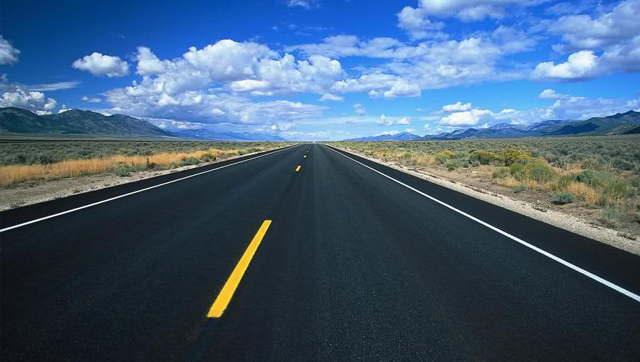
\includegraphics[width=0.4\textwidth]{img/road.jpg}%{./Pictures/mainscreen1.png}
    \caption{Widok z przedniej kamery w samochodzie}
    \label{rys:road}
  \end{center}
  \vspace{-20pt}
  \vspace{1pt}
\end{wrapfigure} 

Do wykrywania pasów ruchu wybraliśmy transformatę Hougha, jako że pasy drogowe widziane z przedniej kamery w aucie najczęściej są zbliżone do linii prostych. Przykład analizowanego obrazu przedstawia rysunek \ref{rys:road}.

Transformata Hougha jest złożoną operacją, którą trudno zrealizować w czasie rzeczywistym na systemie procesorowym. Wpływa na to konieczność wykonania obliczeń dla każdego kąta $\theta$ dla każdego piksela obrazu (lub przynajmniej pikseli należących do krawędzi). Przy obliczaniu transformaty Hougha dla kątów co 1\degree  dla obrazu HD 1280x720 pikseli, trzeba wykonać 331 776 000 mnożeń dla każdej ramki.
Praca \cite{hardware-accelerator} podaje sposób zrównoleglenia obliczeń arytmetycznych w transformacie Hougha na układzie FPGA.


\begin{figure}[!htb]
  \begin{center}
    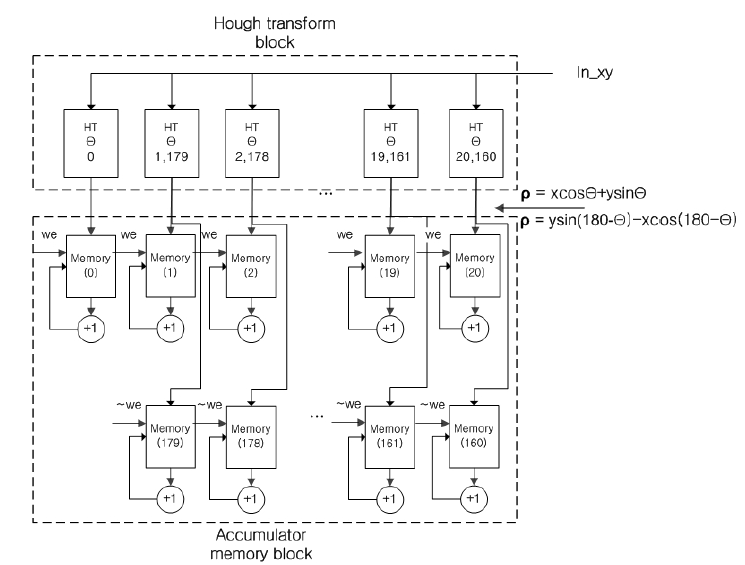
\includegraphics[width=0.9\textwidth]
    {img/hough-accelerator.PNG}
  \end{center}
  \caption{Architektura obliczeniowa transformaty Hougha w pracy \cite{hardware-accelerator}}
  \label{rys:accelerator}
\end{figure}

\newpage

W pracy \cite{kapruziak} opisano 

\blindtext

%\begin{figure}[!htb]
%  \begin{center}
%    \includegraphics[width=14.5cm,trim=1.6cm 6.9cm 1.7cm 8.5cm,clip]
%    {img/exp_omega.pdf}
%  \end{center}
%  \caption{Eksperyment wyznaczenia charakterystyk prędkości śmigieł od napięcia na silnikach przy zablokowanych osiach}
%  \label{plot:exp1}
%\end{figure}





